% !TEX root = ../main.tex
%
% 示例章节：演示模板全部特性
%

\section{引言}

\subsection{基本文字}

这里是正文内容。你可以在这里开始撰写论文\cite{sample2024}。

本文用到的模板特性包括：公式排版、三线表、算法伪代码、定理环境、代码高亮、子图排列等。交叉引用请用 \verb|\autoref|，如 \autoref{tab:sample}、\autoref{fig:sidebyside}、\autoref{eq:energy}。

\subsection{数学公式}

行内公式 $E = mc^2$，独立公式如 \autoref{eq:energy}：

\begin{equation}
    \frac{\partial u}{\partial t} = \alpha \nabla^2 u \label{eq:energy}
\end{equation}

多行对齐：

\begin{align}
    \dot{x} & = \sigma(y - x) \\
    \dot{y} & = \rho x - y - xz \\
    \dot{z} & = -\beta z + xy
\end{align}

约束条件块（empheq）：

\begin{empheq}[left=\empheqlbrace]{flalign}
    & \sum_{j=1}^{n} a_{ij} x_j \leq b_i, \quad i = 1,\dots,m \\
    & x_j \geq 0, \quad j = 1,\dots,n
\end{empheq}

数学算子 \verb|\arcsinh|、\verb|\argmin|、\verb|\sgn|：

\begin{equation}
    \hat{\theta} = \argmin_{\theta} \sum_{i=1}^{n} \|y_i - f_\theta(x_i)\|^2
\end{equation}

\subsection{定理环境}

\begin{Theorem}[均值不等式]
    对于任意非负实数 $a_1, a_2, \dots, a_n$，有
    \begin{equation}
        \frac{a_1 + a_2 + \cdots + a_n}{n} \geq \sqrt[n]{a_1 a_2 \cdots a_n}
    \end{equation}
\end{Theorem}

\begin{Lemma}
    若 $f$ 在 $[a,b]$ 上连续，则 $f$ 在 $[a,b]$ 上有界。
\end{Lemma}

\begin{Definition}
    设 $X$ 是一个非空集合，$\mathcal{T}$ 是 $X$ 的子集族，若 $\mathcal{T}$ 满足……
\end{Definition}

\section{表格}

\autoref{tab:sample} 为三线表示例，使用预定义的 \verb|C|（居中）、\verb|L|（左对齐）、\verb|R|（右对齐）列类型。

\begin{table}[htbp]
    \centering
    \caption{三线表示例}
    \label{tab:sample}
    \begin{tabularx}{0.8\textwidth}{lCCC}
        \toprule
        方法 & 准确率 & 召回率 & F1 值 \\
        \midrule
        SVM      & 92.34\% & 91.02\% & 91.68\% \\
        随机森林 & 94.56\% & 93.78\% & 94.17\% \\
        CNN      & \textbf{96.12\%} & \textbf{95.45\%} & \textbf{95.78\%} \\
        \bottomrule
    \end{tabularx}
\end{table}

斜线表头（diagbox）：

\begin{table}[htbp]
    \centering
    \caption{斜线表示例}
    \label{tab:diag}
    \begin{tabular}{|l|c|c|}
        \hline
        \diagbox{结果}{输入} & 正类 & 负类 \\
        \hline
        预测为正 & TP & FP \\
        预测为负 & FN & TN \\
        \hline
    \end{tabular}
\end{table}

\section{算法伪代码}

\begin{algorithm}[htbp]
    \caption{梯度下降法}
    \label{alg:gd}
    \KwInput{学习率 $\eta$，迭代轮数 $T$，初始参数 $\theta_0$}
    \KwOutput{最优参数 $\theta^*$}
    $t \gets 0$\;
    \While{$t < T$}{
        计算梯度 $g_t = \nabla L(\theta_t)$\;
        更新参数 $\theta_{t+1} \gets \theta_t - \eta g_t$\;
        $t \gets t + 1$\;
    }
    \Return{$\theta_T$}
\end{algorithm}

\section{图片与子图}

使用 subcaption 宏包排布子图（\autoref{fig:sidebyside}）：

\begin{figure}[htbp]
    \centering
    \begin{subfigure}[b]{0.45\textwidth}
        \centering
        % \includegraphics[width=\textwidth]{figures/example-a}
        \caption{子图 A}
        \label{fig:suba}
    \end{subfigure}
    \hfill
    \begin{subfigure}[b]{0.45\textwidth}
        \centering
        % \includegraphics[width=\textwidth]{figures/example-b}
        \caption{子图 B}
        \label{fig:subb}
    \end{subfigure}
    \caption{并排子图示例}
    \label{fig:sidebyside}
\end{figure}

\section{代码高亮}

\begin{lstlisting}[language=Python, caption=Python 代码示例]
import numpy as np

def softmax(x):
    """Compute softmax values for each row."""
    e_x = np.exp(x - np.max(x, axis=1, keepdims=True))
    return e_x / e_x.sum(axis=1, keepdims=True)
\end{lstlisting}

\section{TikZ 绘图与带圈数字}

带圈数字（pifont + tikz）：

\ding{172} \ding{173} \ding{174} \ding{175} \ding{176} \quad
\circled{1} \circled{2} \circled{3} \circled{4} \circled{5}

TikZ 示意图：

\begin{center}
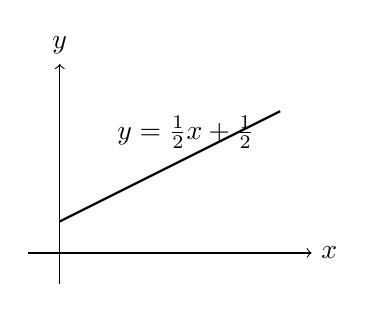
\begin{tikzpicture}[scale=0.8]
    \draw[->] (-0.5,0) -- (4,0) node[right] {$x$};
    \draw[->] (0,-0.5) -- (0,3) node[above] {$y$};
    \draw[domain=0:3.5, smooth, thick] plot (\x, {0.5*\x + 0.5});
    \node[above] at (2,1.5) {$y = \frac{1}{2}x + \frac{1}{2}$};
\end{tikzpicture}
\end{center}

\section{列表}

有序列表：

\begin{enumerate}[label=\arabic*.]
    \item 数据预处理
    \item 特征提取
    \item 模型训练
    \item 结果评估
\end{enumerate}

自定义标签列表：

\begin{enumerate}[label=\textbf{Step \arabic*:}, leftmargin=*]
    \item 加载数据集
    \item 划分训练集和测试集
    \item 训练分类器
\end{enumerate}
